\section{Numerical experiments}
\label{sec:ct-experiments}

We compare minibatch and full-batch SFRAMES with
SPRING--SARAH~\cite{spring}, ProxSARAH~\cite{proxsarah}, and PALM~\cite{palm}
on low-rank reconstruction from real low-dose computed tomography (CT)
data. The experiment examines data fitting and constraint satisfaction at
equal gradient-view budgets.

\paragraph{Reconstruction problem.}
The negative logarithm of calibrated X-ray transmission approximates line
integrals of attenuation. A \emph{view} groups detector rays at one source
angle. For an image \(X\), the linear forward map for view \(i\) is
\([P_i(X)]_j=\sum_{p,q}\ell_{ij,pq}X_{pq}\), where \(\ell_{ij,pq}\) is
the length of ray \(j\) through pixel \((p,q)\). Its adjoint \(P_i^\ast\)
backprojects detector residuals onto the image using the same weights.

We use low-dose fan-beam measurements from 2DeteCT~\cite{detect} and
represent the \(512\times512\) attenuation image as \(UV^\top\), with
\(U,V\in\mathbb R^{512\times64}\). For a set \(\mathcal I\) of \(N\)
training views and detector data \(y_i\in\mathbb R^d\), \(d=956\), the
training loss is
\begin{equation}
  f(U,V)=\frac1N\sum_{i\in\mathcal I}
          \frac{\|P_i(UV^\top)-y_i\|_2^2}{2d}.
  \label{eq:ct-loss}
\end{equation}
We constrain each factor by a spectral norm bound and require nonnegative
factors, which ensure nonnegative attenuation. For \(x=(U,V)\), set
\[
 C=\{(U,V):\|U\|_{\rm op}\le R_U,\ \|V\|_{\rm op}\le R_V\},
 \qquad D=\{(U,V):U\ge0,\ V\ge0\}.
\]
The bilinear factorization makes the problem nonconvex. Its SFRAMES
formulation is \(\min_{x\in C} f(x)+g(Tx)\), with
\(T=\operatorname{Id}\) and \(g=\iota_D\), the indicator of \(D\).
Uniformly sampling views gives an unbiased estimator of \(\nabla f\).
The spectral-ball linear oracle separates by factor and uses one thin SVD
per block. The gradient of the Moreau envelope of \(g\) is
\((x-x_+)/\beta\), where \(x_+\) clips both factors to nonnegativity.

\paragraph{Evaluation.}
We evaluate on 14 slices from six acquisition groups, with either \(360\)
or \(1{,}080\) training views and \(360\) held-out views per slice.
The two view counts change the finite-sum size while keeping the factor
dimensions fixed. We use three stochastic repetitions per slice and view
count, with a common initialization across methods.
We compare the last iterate within \(69{,}120\) gradient forward and
adjoint views per direction, including snapshots and recursive differences.
Curvature-estimation views are recorded separately and excluded from this cap.
A gradient call evaluates one joint or block gradient on a batch.
All trajectories use observations recorded at every update.

Raw loss is the data-fit term \(f\) evaluated at the current factors.
To assess a feasible reconstruction, we clip each factor to
nonnegativity and rescale it radially into its spectral ball if needed.
We evaluate the resulting image by training and held-out loss and relative
Frobenius error against the high-dose reconstruction.
Repair is used only for evaluation. Raw nonnegativity violation is
\[
 d_D(U,V)=\bigl(\|U-U_+\|_F^2+\|V-V_+\|_F^2\bigr)^{1/2}.
\]
Relative infeasibility divides \(d_D\) by
\(\bigl(\|U_0\|_F^2+\|V_0\|_F^2\bigr)^{1/2}\).
Quality summaries take successive medians over repetitions, slices within
each group, and groups. Paired percentage changes are computed before this
aggregation, so they need not equal ratios of the table entries.

\paragraph{Results.}
At \(N=360\), paired repaired loss relative to ProxSARAH
is \(13.4\%\) lower for loss-tuned SFRAMES and \(12.6\%\) lower for the joint tune.
The group-balanced fractions meeting both the \(30\%\) relative-loss
and \(1\%\) raw-feasibility targets are \(92\%\),
\(0\%\), and \(100\%\) for the joint tune,
loss-tuned SFRAMES, and ProxSARAH, respectively.

At \(N=1{,}080\), paired repaired loss relative to ProxSARAH
is \(21.0\%\) lower for loss-tuned SFRAMES and \(21.2\%\) lower for the joint tune.
The group-balanced fractions meeting both the \(30\%\) relative-loss
and \(1\%\) raw-feasibility targets are \(92\%\),
\(0\%\), and \(94\%\) for the joint tune,
loss-tuned SFRAMES, and ProxSARAH, respectively.

Relative to the former cap on total views, the paired repaired-loss changes are \((-36.1\%,-25.5\%)\) for PALM and \((-32.3\%,-25.6\%)\) for SPRING--SARAH at \(N=360,1{,}080\), respectively. Including curvature, total views are \(7.0\times\) gradient views for PALM and \(3.6\times,2.9\times\) for SPRING--SARAH. All proximal baselines remain nonnegative. This comparison uses equal gradient work.
Table~\ref{tab:ct-results} gives endpoint metrics; Figures~\ref{fig:ct-trajectories-360}
and~\ref{fig:ct-trajectories-1080} show progress versus iterations, gradient calls,
and gradient views.

\begin{table}[!htbp]
\centering
\caption{Endpoint quality at a common gradient-view budget; curvature work is excluded from this cap. The three loss columns are multiplied by \(10^3\). Held-out loss and reference error use the repaired image. Infeasibility is relative to the initial factor-pair norm, in percent. Bold marks the best value within each view count.}
\label{tab:ct-results}
\small
\setlength{\tabcolsep}{4pt}
\begin{tabular}{@{}llrrrrr@{}}
\toprule
$N$ & Method & Raw & Repaired & Held-out & Ref. error & Infeas.\ (\%) \\
\midrule
360 & Minibatch SFRAMES (original) & $\boldsymbol{5.66}$ & $\boldsymbol{6.11}$ & $\boldsymbol{6.49}$ & $0.362$ & $2.03$ \\
360 & Minibatch SFRAMES (joint tune) & $6.39$ & $6.48$ & $6.65$ & $\boldsymbol{0.317}$ & $0.67$ \\
360 & Full-batch SFRAMES & $6.34$ & $6.99$ & $7.14$ & $0.333$ & $3.06$ \\
360 & SPRING--SARAH & $12.78$ & $12.78$ & $12.81$ & $0.496$ & $\boldsymbol{0.00}$ \\
360 & ProxSARAH-v3 & $7.93$ & $7.93$ & $7.99$ & $0.376$ & $\boldsymbol{0.00}$ \\
360 & PALM & $13.60$ & $13.60$ & $13.68$ & $0.513$ & $\boldsymbol{0.00}$ \\
1{,}080 & Minibatch SFRAMES (original) & $\boldsymbol{5.82}$ & $\boldsymbol{6.22}$ & $\boldsymbol{6.32}$ & $\boldsymbol{0.283}$ & $2.01$ \\
1{,}080 & Minibatch SFRAMES (joint tune) & $6.46$ & $6.55$ & $6.58$ & $0.286$ & $0.67$ \\
1{,}080 & Full-batch SFRAMES & $7.85$ & $8.90$ & $8.87$ & $0.365$ & $4.51$ \\
1{,}080 & SPRING--SARAH & $14.27$ & $14.27$ & $14.31$ & $0.524$ & $\boldsymbol{0.00}$ \\
1{,}080 & ProxSARAH-v3 & $8.77$ & $8.77$ & $8.76$ & $0.403$ & $\boldsymbol{0.00}$ \\
1{,}080 & PALM & $20.01$ & $20.01$ & $20.03$ & $0.580$ & $\boldsymbol{0.00}$ \\
\bottomrule
\end{tabular}
\end{table}

\paragraph{Implementation and parameter selection.}
All methods start from a nonnegative SVD-based factorization of a
sensitivity-normalized backprojection of training views, with its
amplitude fitted to those views. Set
\(R_U=2\|U_0\|_{\rm op}\) and \(R_V=2\|V_0\|_{\rm op}\).
Minibatch SFRAMES samples \(64\) views uniformly without replacement,
independently across iterations; full-batch SFRAMES uses all \(N\) views.
Both use \(\gamma_k=\gamma_0(k+1)^{-3/4}\),
\(\alpha_k=(k+1)^{-1/2}\) for gradient averaging, and
\(\beta_k=\beta_0(k+1)^{-1/4}\), with
\(\beta_0=c_\beta/\max(L_U,L_V)\) scaled by initial block-curvature estimates.
The loss-tuned SFRAMES setting \((c_\beta,\gamma_0)=(16,0.1)\)
is selected jointly by repaired training loss on two development slices.
A second sweep selects \((c_\beta,\gamma_0)=(4,0.1)\) using the joint
endpoint target of repaired loss at most \(30\%\) of its initial value
and relative orthant distance at most \(1\%\).
The two searches use \(8{,}640\) and \(34{,}560\) views per direction,
respectively. No evaluation slice enters parameter selection.

SPRING--SARAH uses \(64\)-view differences, independent full-gradient
refreshes with probability \(1/16\), and steps \(1/(2\widetilde L)\).
PALM uses full block gradients and steps \(1/\widehat L\).
Both retain their original steps and sampling rules during continuation.
They estimate current block curvature by five power iterations followed
by a final norm evaluation, using minibatches for SPRING and all views for PALM.
ProxSARAH uses the paper's constant-parameter variant v3: full snapshots,
relaxation \(0.99\), and \((b,m)=(27,18)\) or \((48,32)\) at the two
view counts. Its proximal step is \(0.400802/\widehat L\), with
\(\widehat L=0.25(L_U+L_V)\); only this curvature-scale multiplier
is selected on the development slices at \(34{,}560\) views per direction.
These practical curvature estimates are not certified Lipschitz bounds.
All three baselines project each factor onto its spectral ball intersected
with the nonnegative orthant. The \CTReproducibility{} specifies the data split,
preprocessing, search grids, and numerical solver settings.

\begin{figure}[!htbp]
 \centering
 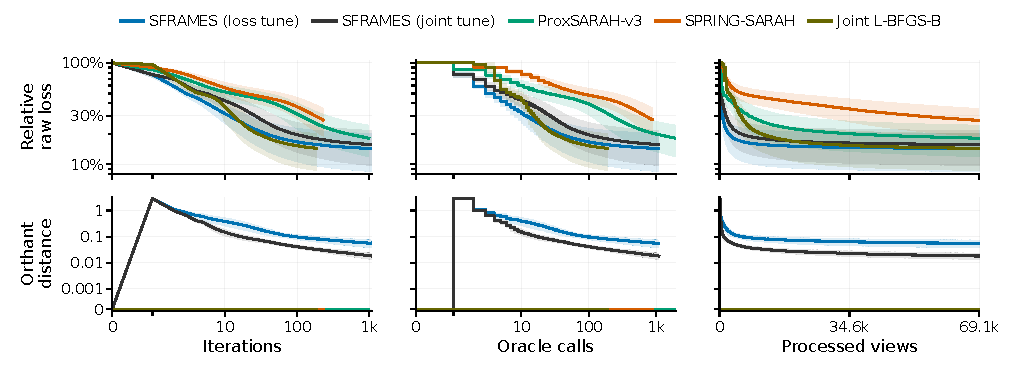
\includegraphics[width=\linewidth]{trajectories_360.pdf}
 \caption{Mean trajectories for \(N=360\), with shaded bands showing
 \(\pm1\) standard deviation over runs and slices, weighting acquisition
 groups equally. Gradient-work summaries use the latest recorded iterate
 within each budget; curves stop at the range shared by all runs of a method.
 Training losses are relative to initialization. Vertical markers indicate
 one quarter of the gradient-view budget.}
 \label{fig:ct-trajectories-360}
\end{figure}

\begin{figure}[!htbp]
 \centering
 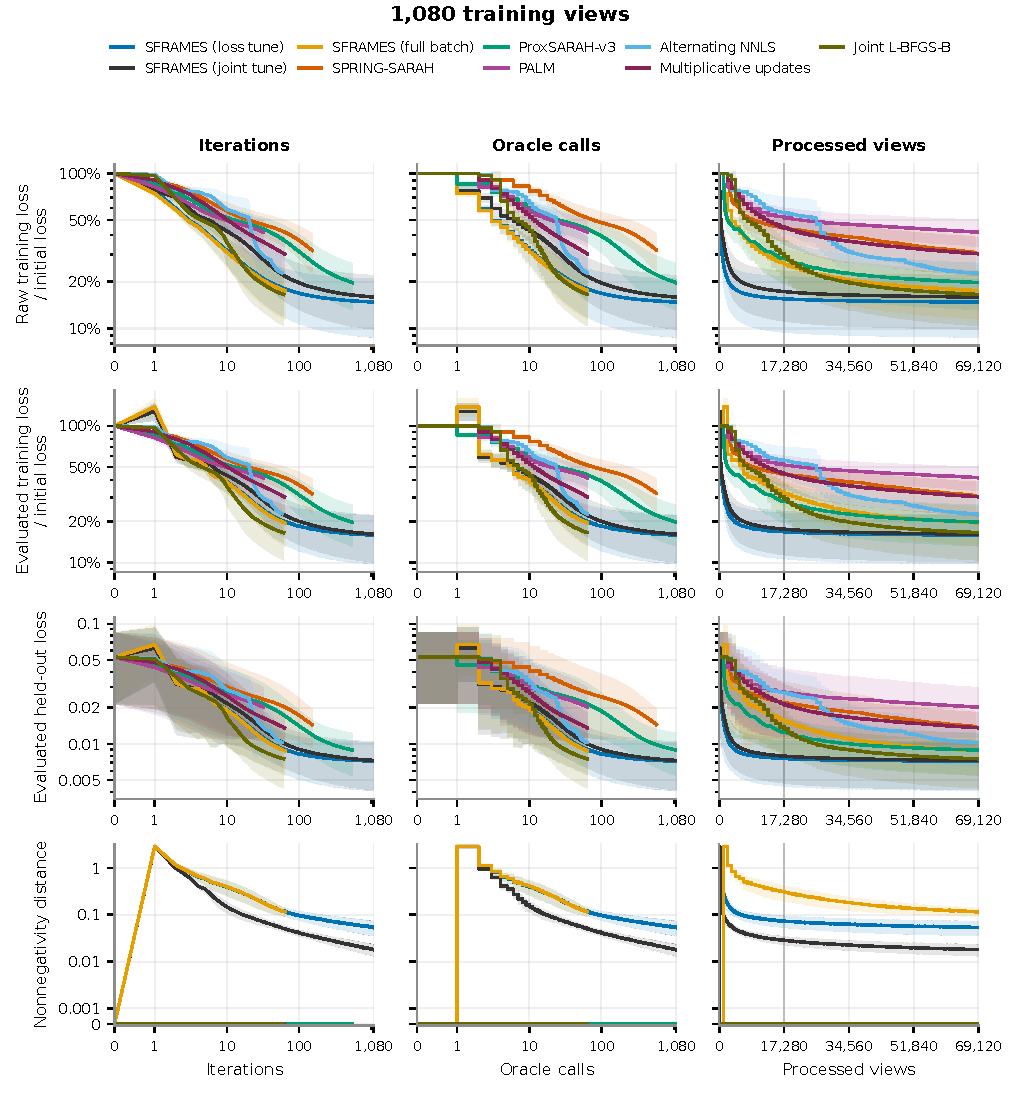
\includegraphics[width=\linewidth]{trajectories_1080.pdf}
 \caption{Mean trajectories and \(\pm1\) standard-deviation bands for \(N=1{,}080\), as in
 Figure~\ref{fig:ct-trajectories-360}. The three projection baselines
 coincide at zero orthant distance.}
 \label{fig:ct-trajectories-1080}
\end{figure}
